\documentclass[draftclsnofoot, onecolumn, letterpaper,10pt,compsoc]{IEEEtran}

\usepackage{url}
\usepackage{color}
\usepackage{hyperref}
\hypersetup{
    colorlinks=true,
    linkcolor=blue,
    filecolor=magenta,      
    urlcolor=blue,
}
\usepackage{geometry}
\usepackage{tabularx}
\usepackage{listings}
\usepackage{fancyvrb}
\usepackage{varwidth}
\usepackage{setspace}
\usepackage{float}
\usepackage{caption}
\usepackage{graphicx}
\usepackage{pgfgantt}
\graphicspath{ {./images/} }

\geometry{margin=0.75in}   
\singlespacing

\def \TitlePageHeader{Droplet Productions}
\def \TitlePageTitle{Progress Report}
\def \GroupNumber{by Group 13}
\def \GroupMembers{James Barry, Tarren Engberg, Dennis Li, James Luo,  Brice Ng}
\def \CourseTitle{CS 462 - Senior Design}
\def \CourseTerm{Winter 2018}

\title{Group13ProgressReport}
			
\newcommand{\NameSigPair}[1]{\par
\makebox[2.75in][r]{#1} \hfil 	\makebox[3.25in]{\makebox[2.25in]{\hrulefill} \hfill		\makebox[.75in]{\hrulefill}}
\par\vspace{-12pt} \textit{\tiny\noindent
\makebox[2.75in]{} \hfil		\makebox[3.25in]{\makebox[2.25in][r]{Signature} \hfill	\makebox[.75in][r]{Date}}}}
\renewcommand{\NameSigPair}[1]{#1}


%i pull \centerfloat from memoir here, so i can use it for figures
\makeatletter
\newcommand*{\centerfloat}{%
  \parindent \z@
  \leftskip \z@ \@plus 1fil \@minus \textwidth
  \rightskip\leftskip
  \parfillskip \z@skip}
\makeatother


\begin{document}
\begin{titlepage}
    \pagenumbering{gobble}
    \begin{singlespace}
        \hfill    
        \par\vspace{.2in}
        \centering
        \scshape{
            \huge \TitlePageHeader \par
            {\large\today}\par
            \vspace{.5in}
            \textbf{\Huge \TitlePageTitle }\par
            \vfill
            \vspace{5pt}

            \vspace{5pt}
            {\Large
                \NameSigPair{\GroupNumber}\par
            	\NameSigPair{\GroupMembers}\par
                \NameSigPair{\CourseTitle}\par
                \NameSigPair{\CourseTerm}\par
            }
            \vspace{20pt}
        }
    \end{singlespace}
    \begin{abstract}
    This document is a review of Group 13's progress in developing Droplet during Winter term. The document includes a recap of the project's purpose, a report on the Group's current progress, an overview of the remaining work, and a description of the problems encountered during development along with their respective solutions, if any.
    \end{abstract}
\end{titlepage}

\newpage
\pagenumbering{arabic}
\clearpage

\pagebreak

\section{Project Purposes and Goals Recap}
The project is a location-tagging mobile application called Droplet. Its goal is to bring physical connection to social media by making people explore the world to see posts made by others. The project attempts to achieve this goal by attaching a user's posts to a location instead of just to their account. In addition, only nearby users can view and interact with those posts. By limiting interactions to posts made within someone's general vicinity, it filters out information that a user cannot physically interact with while encouraging users to actively search for posts via exploration.

\section{Current Progress}
\subsection{Database}
The team has created a MongoDB server using an automated cloud service, and has successfully connected to the database.  In addition, back-end endpoints have been created for post and comment CRUD (Create, Read, Update, and Delete) functionality.  Posts have the option of being text, a picture, or a combination of both.  Below is a snippit of code from the post schema Droplet has implemented.  This schema details what information the post will consist of, and what types the fields accept.
\small{
\begin{lstlisting}[caption=Post Schema]
const postSchema = new mongoose.Schema({
    _id: mongoose.Schema.Types.ObjectId,
    username: {
        type: String,
        ref: 'User',
        required: 'Username is required'
    },
    content: {
        type: String
    },
    postImage: {
        type: String,
        default: undefined
    },
//    splash_rad: Number,
    comments: [{
        type: mongoose.Schema.Types.ObjectId,
        ref: 'Comment',
        required: 'Comment is required'
    }],
    created: {
        type: Date,
        default: Date.now
    },
    updated: {
        type: Date,
        default: Date.now
    },
    likes: [{
        type: mongoose.Schema.Types.ObjectId,
        ref: 'User'
    }],
    location: {
        type: {
            type: String,
            default: "Point",
            required: true
        },
        coordinates: {
            type: [],
            required: true
        }
    },
    userid: {
        type: mongoose.Schema.Types.ObjectId,
        ref: 'User'
    }
});
\end{lstlisting}
}
The back-end currently allows for users to be created and deleted, each with a unique username, a hashed password, and an automatically generated unique ID.  These users can create posts, with each post structured as above.  The location field currently takes a GeoJSON input, consisting of a type and a coordinate pair.  To search for nearby posts, the team has utilized a built-in function MongoDB offers called \textit{geoNear}.  The function will search through the posts document in the database and compare each post location to the user's coordinates.  It then returns a sorted array of all posts within a specified radius.  \textit{GeoNear} also uses a spherical index when calculating distances between coordinates rather than a flat plane to better model the post's location.  Below is an example of the function used.
\small{
\begin{lstlisting}[caption=Get Nearby Posts]
Post.aggregate([
        {
            $geoNear: {
                near: { type: "Point", coordinates: [lng, lat] },
                distanceField: "dist.calculated",
                key: "location",
                includeLocs: "dist.location",
                maxDistance: 10,
                spherical: true
            }
        }
    ])
\end{lstlisting}
}\newline

As mentioned earlier, each post has a comment array to be filled with ID's of comments and a likes array to be filled with userID's of users who liked the post.  Below is the code used to like a post.  This first checks to see if a user has already liked a post by checking to see if the username is in the 'like' array.  If they have, then they cannot duplicate the like.  If the username is not in the array, then it is appended to the end and the array is updated.  Every other scenario generates an appropriate error.
\small{
\begin{lstlisting}[caption=Liking a Post]
//Check if user has already liked the post
    Post.find( { "_id" : Pid, likes: {$in: [Uid] }  }, (err, post) => {
        if(err) {
            return res.status(500).send(err);
        }
        //Already liked the post
        else if(post.length > 0 ) {
            return res.status(401).json({
                success: "You have already liked this post!"
            });
         }
        else {
            //Like the post
            Post.updateOne({ "_id" : Pid}, {$push: { likes: Uid}}, (err, post) => {
                if(err) {
                    return res.status(500).send(err);
                }
                else {
                    return res.status(200).json({
                        success: 'You have liked this post!'
                    });
                }
            });
        }
    });
\end{lstlisting}
}
The team has also implemented cascading deletion for database maintenance.  An example of this is when a user is deleted; the user's comments, posts, and people's comments on those posts are all deleted.  Without cascading deletion, only the user would be deleted, and none of their content, leaving floating data in the database.  With cascading deletion, the database frees up memory for users and helps minimize server slowdown.
\pagebreak
\subsection{Map}
The team has implemented a map into the application using the MapBox API. Currently, they are able to display a basic map onto the screen. This map allows users to click and drag to various locations on the map, and zoom into a specific location. In addition to displaying a map, our team has successfully added markers onto the map at distinct points with their longitude and latitudes. The marker icon has also been changed to the droplet icon to match our initial mock-ups. These markers can be clicked on the display a pop-up of the username and the data attached to the posts. In addition to these UI aspects, the team is able to retrieve user location information and map screen information, which will be critical to deciding which posts to display to the users.

\begin{figure}[!ht]
    \centering
    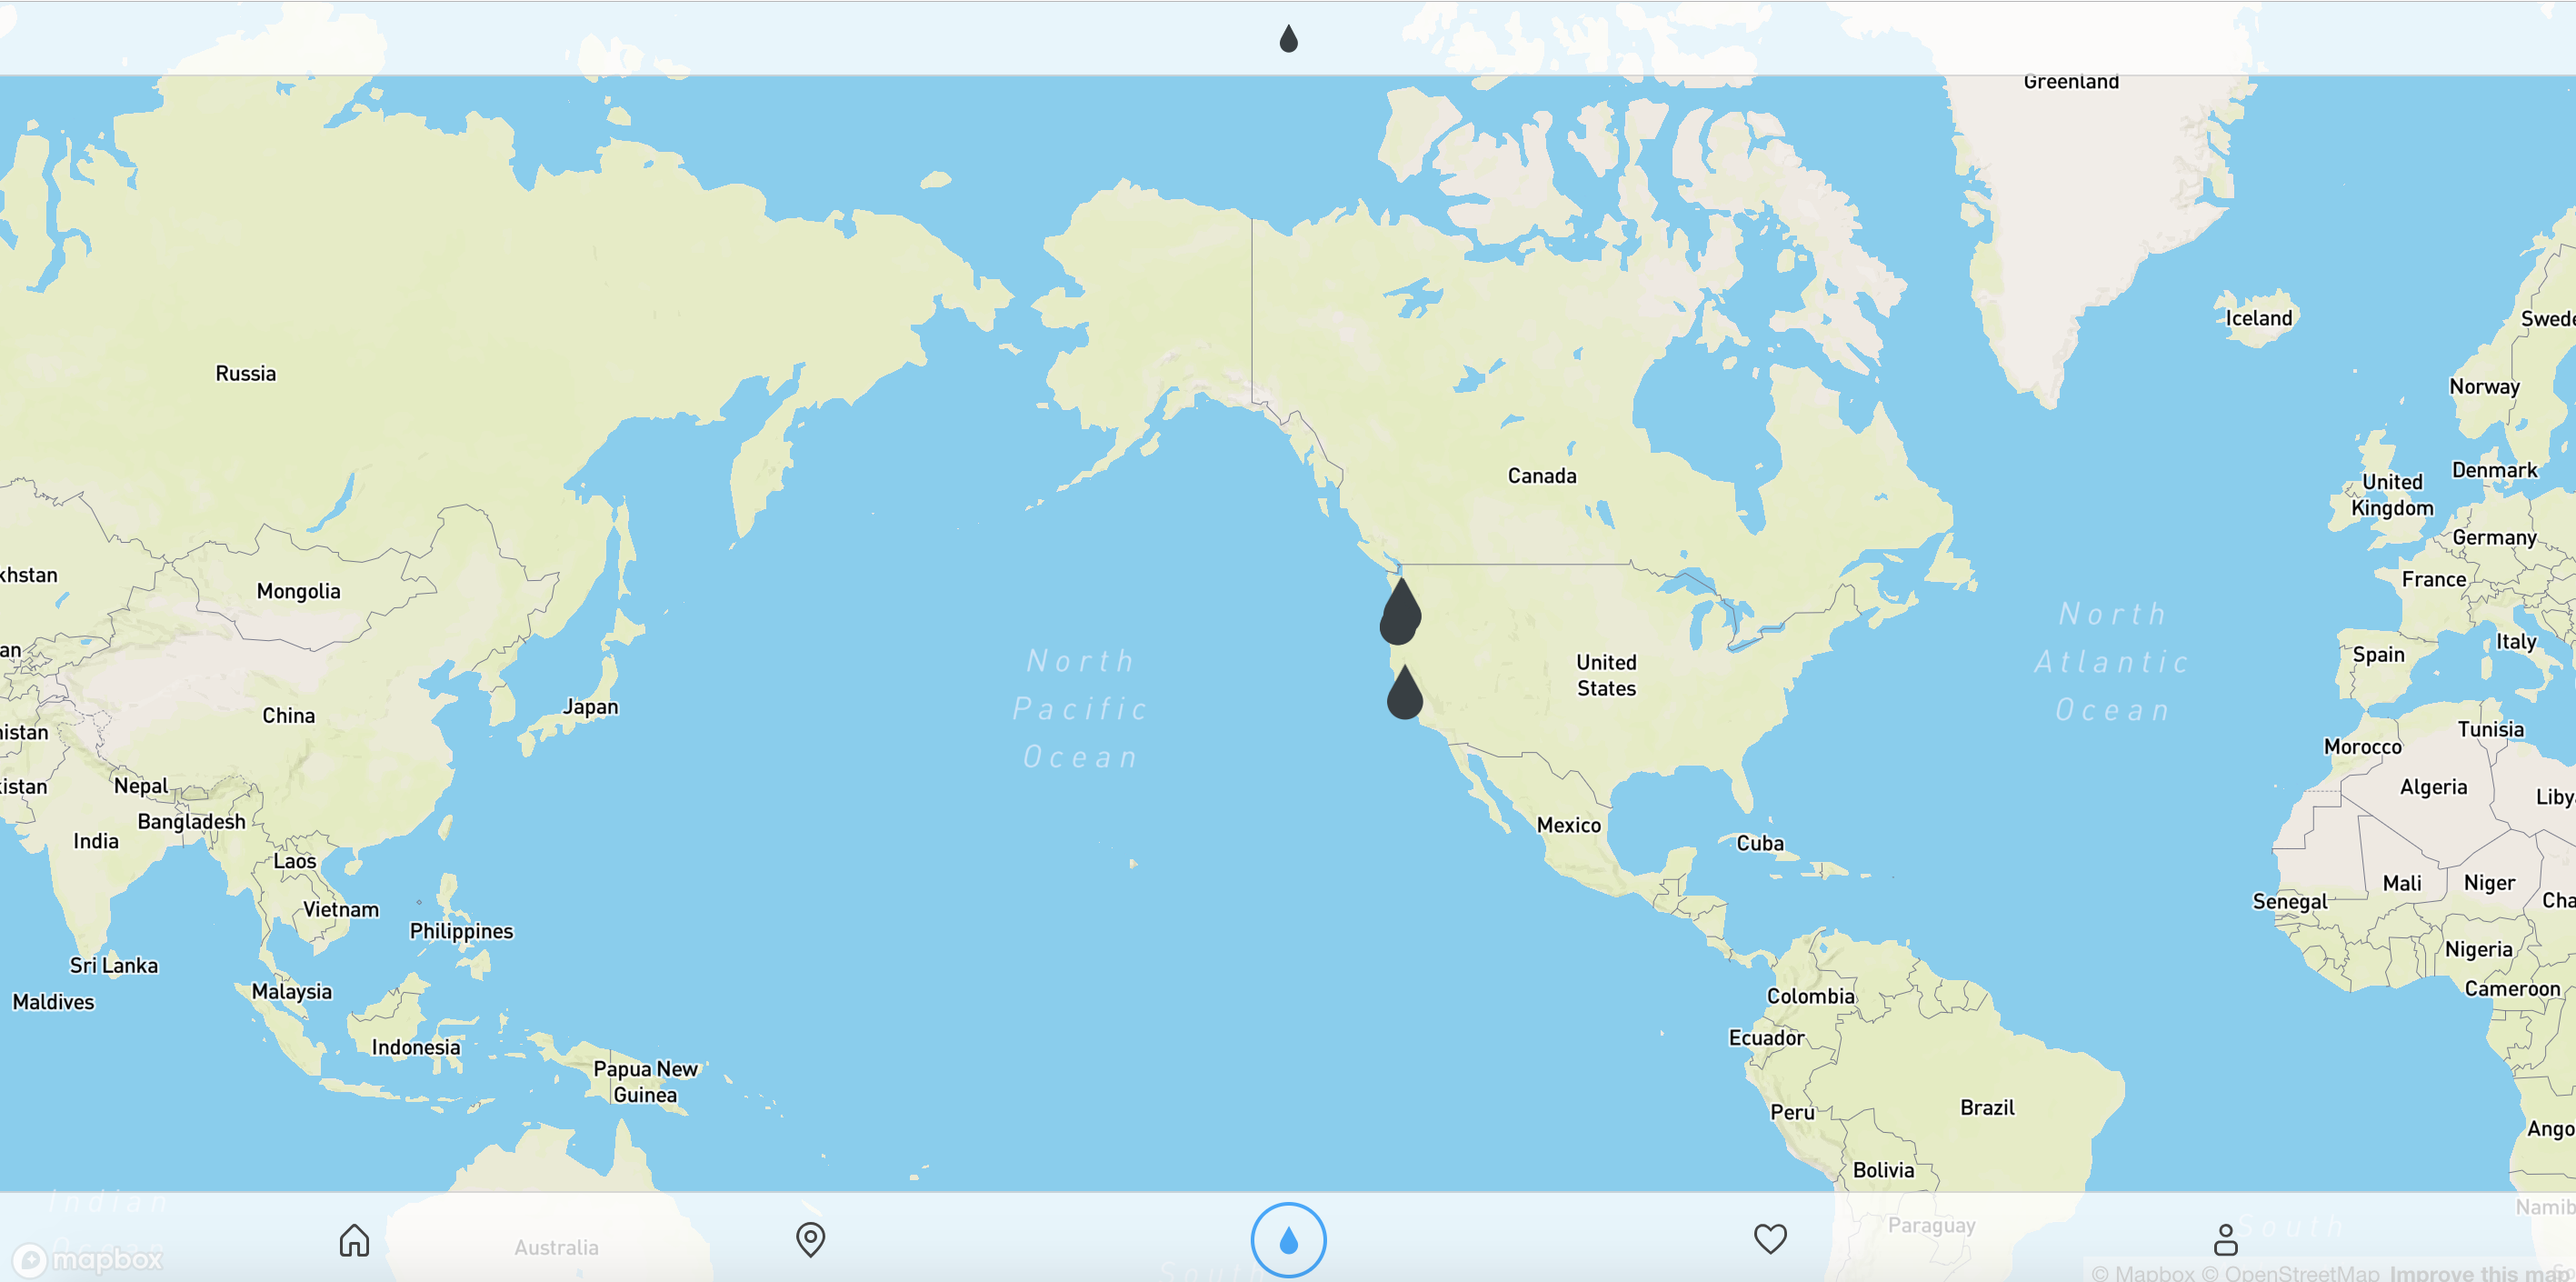
\includegraphics[scale=.25]{images/Map1.png}
    \caption{Map Screen Zoomed Out}
    \label{fig:my_label}
\end{figure}
\begin{figure}[!ht]
    \centering
    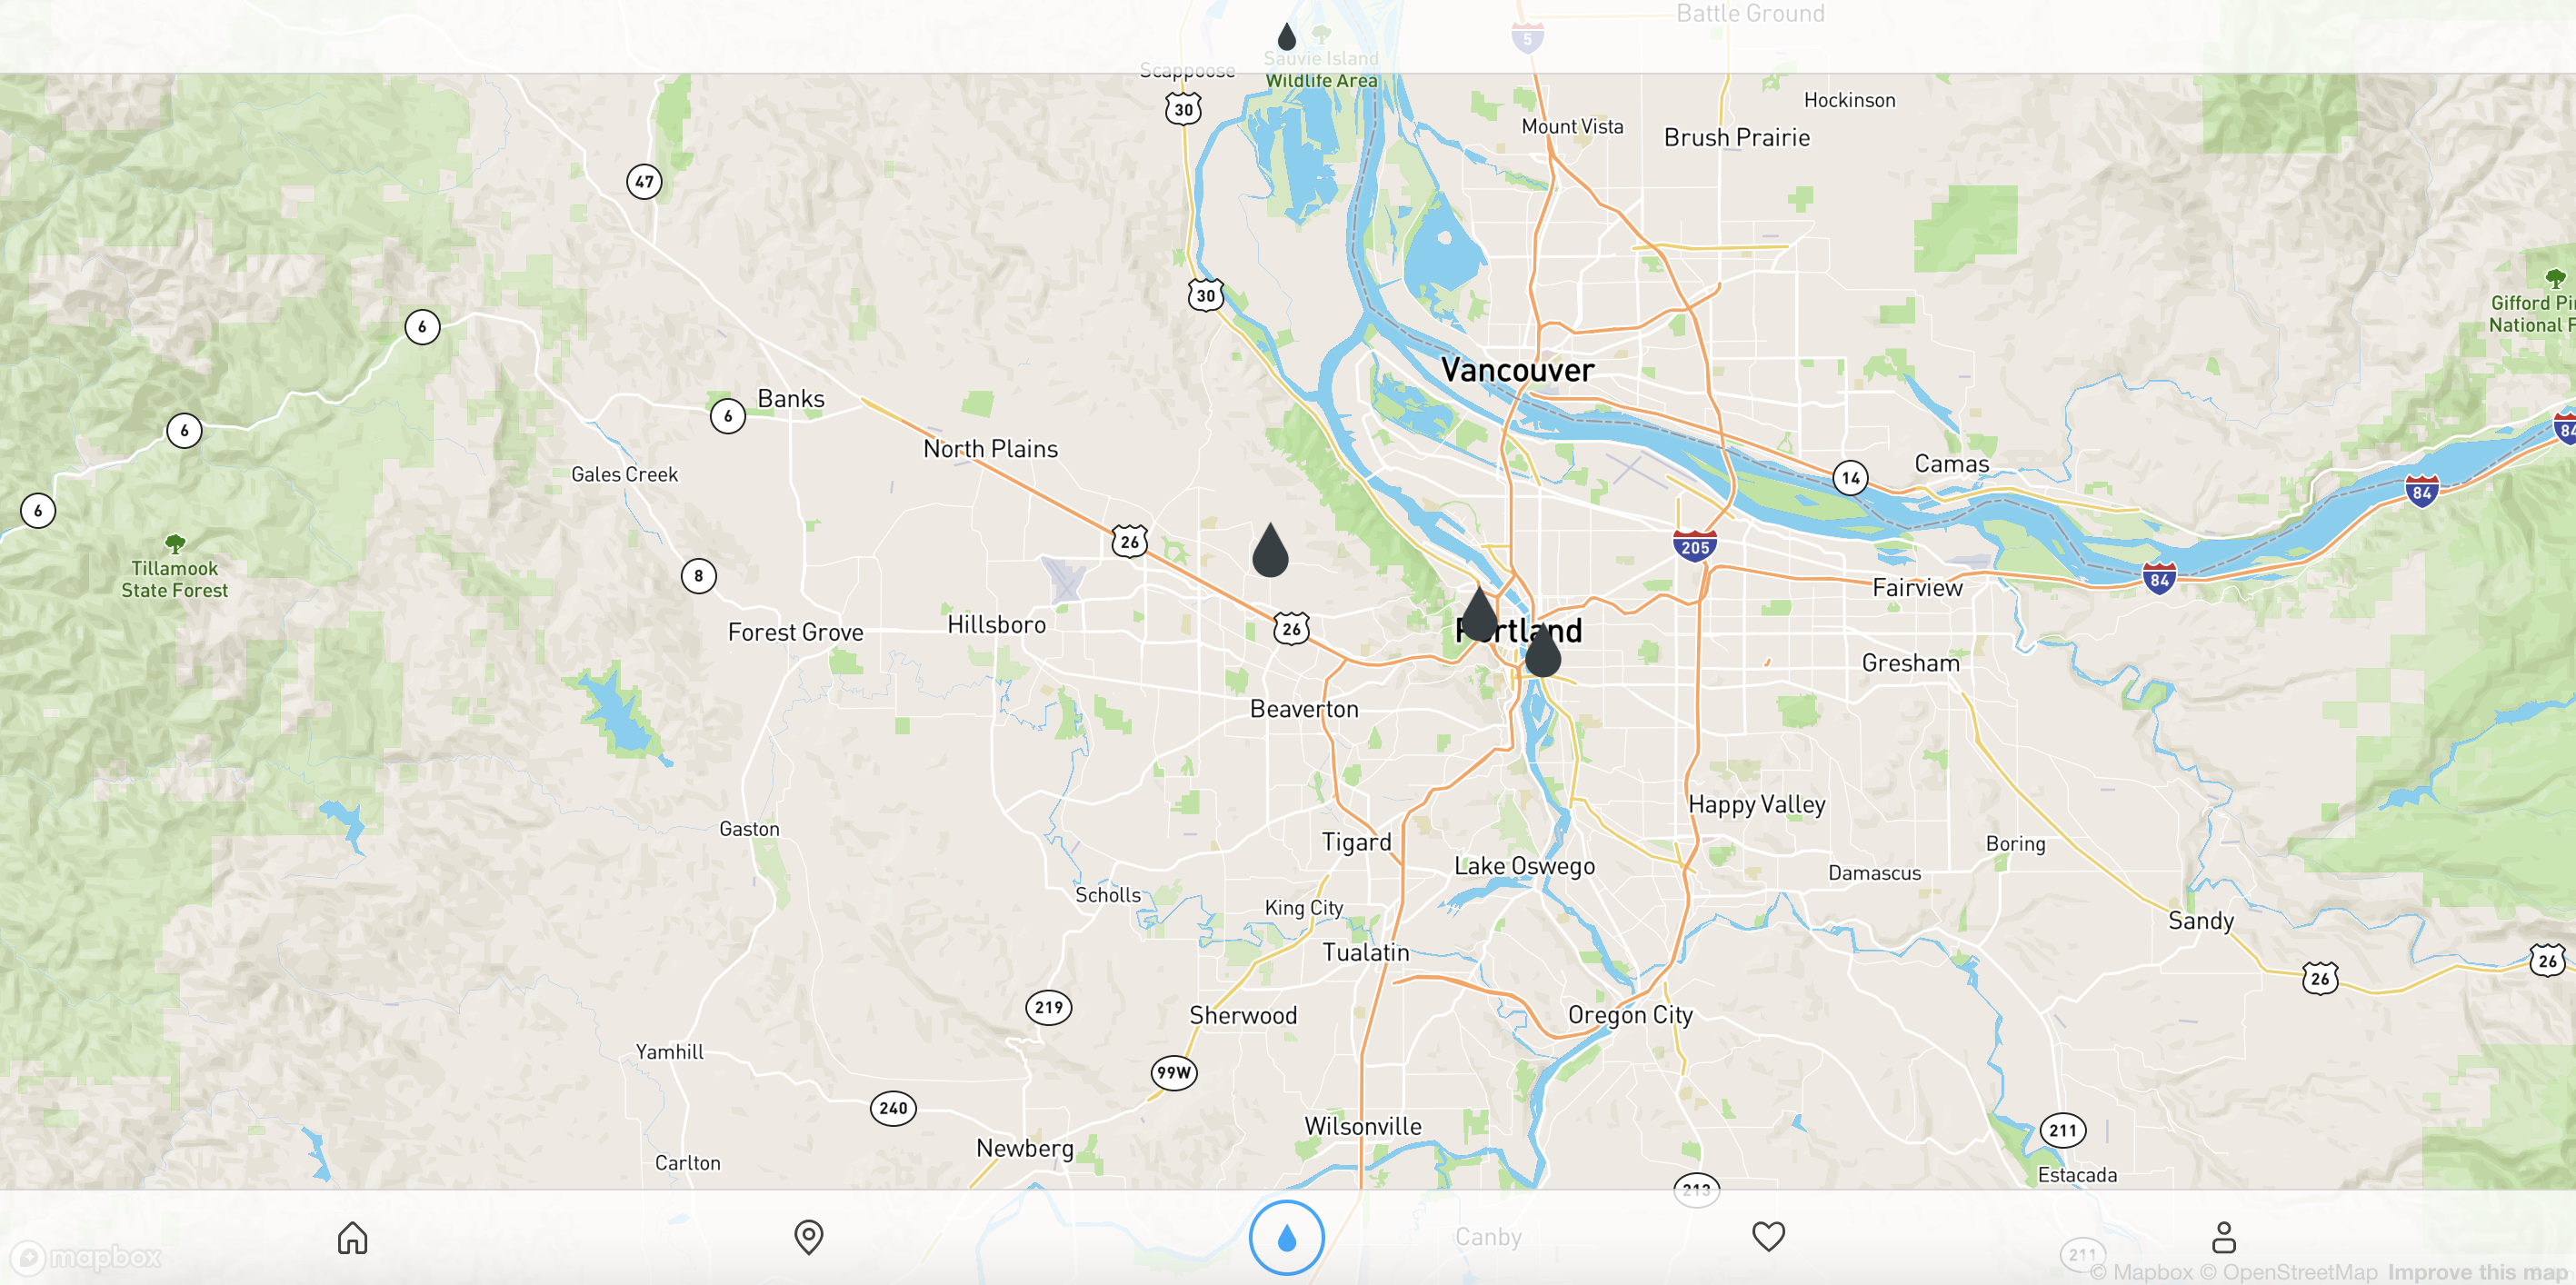
\includegraphics[scale=.25]{images/Map2.png}
    \caption{Map Screen Zoomed In}
    \label{fig:my_label}
\end{figure}

\pagebreak

\subsection{Authentication}
The team has opted to use JSON Web Tokens (JWTs) to handle user authentication, and currently there is a login page that is capable of parsing the user's inputs, sending them to the server, and getting back and storing the server's response in a cookie. The JWTs payload stores the userID, which is a necessary component in several endpoints i.e. the ones for getting the profile information and making a post.

\subsection{Other Client Screens}
The team has managed to integrate the Redux client library to simplify the app state management and enforce a system for subscribing to app state changes that is immutable and functionally scalable. The home page is able to asynchronously fetch post data from the server and display their content in list view. Recent changes have included a reorganization of the navigation hierarchy to make the first three pages, which all have the same dynamic map background, to be considered the home page. Along with these home pages, there are three sub-pages of posts, map-only view and the new-post view. The new-post page is still under construction.

\section{Remaining Work}
\subsection{Database}
Currently, the back-end has user, post, and comment CRUD functionality.  The remaining back-end work that needs to be implemented is the ability to accept location information from the device, in GeoJSON format.  When the map is fully integrated, the team will need to find a way to return that posts that are outside the range, but not reveal information about them.  The goal is to alert the user of posts and encourage them to walk within range.

\subsection{Map}
In the end, the team wants to be able to view posts near users from the map. Currently, the map is not interactive besides being able to drag and zoom the map. The team also wants to be able to add popups that show the posts. In order to implement this we would need to be able to create the popups and connect them with the data from the database. In regards to the style, if the team decides to change the style, the team can implement this through using MapBox API's present styles. In addition, a new style can be created through MapBox Web Studio and integrated into the application. The final aspect we would need to add to our application is requesting user location for the map.

\subsection{Authentication}
There isn't currently any button for logging in, since it's still up in the air exactly how to go about asking the user to login (a small popup, a unique window, should the user be asked to login when they start the app/page, etc.) The UI doesn't update itself to reflect that a user is logged in either (i.e. when logged in, there should be a logout button). 

\subsection{Other}
In addition to the work listed above, there are various elements that still need to be implemented. A page or popup for creating posts still needs to be made, and it will have to be linked to the back-end and send things such as post content and location data to the database. Interacting with posts themselves (not on the map) still needs to be worked on too i.e. comments and likes. 

\section{Problems and Solutions}

\subsection{Big Data and Great Circle Navigation}
An ongoing point of discussion for the group has been how to store and parse information. Since posts are based on locations, they're spattered around in an unstructured way. Organizing these is important, because, as the size of our database approaches infinity, it becomes gradually more time consuming to search the database for posts that are nearby the user. 

An issue that arises from this is managing how to calculate the distance between two lat/long points, since latitude and longitude cannot be directly converted to meters. Both of these problems have been solved before, but determining the best way to balance and solve them for Droplet was a challenge. 

Our ultimate solution was to take advantage of MongoDB's lat/long data type and its geo-near function. These allow us to store information based on its lat/long location, as well as find points that are within a certain meters distance of a given location. This is exactly what we need, and not needing to implement our own solution likely saved a great deal of time. Section 2.1 can be referred to for greater detail on this topic. 


\end{document}
